%%%%%%%%%%%%%%%%%%%%% chapter.tex %%%%%%%%%%%%%%%%%%%%%%%%%%%%%%%%%
%
% sample chapter
%
% Use this file as a template for your own input.
%
%%%%%%%%%%%%%%%%%%%%%%%% Springer-Verlag %%%%%%%%%%%%%%%%%%%%%%%%%%

\chapter{Maximum-Likelihood and Bayesian Parameter Estimation}\label{tecnicheParametriche}
\section{Introduzione}
Nella sezione \ref{teoriaBaesiana} abbiamo visto come progettare un classificatore conoscendo le probabilità a priori $P(\omega_i)$ e le funzioni di distribuzione di probabilità condizionate $p(\mathbf{x}|\omega_i)$. Sfortunatamente, nei problemi di pattern recgnition non sempre abbiamo una conoscenza completa della struttura probabilistica. Nel caso tipico abbiamo una vaga conoscenza della situazione insieme al numero dei dati di \emph{training}. Il problema è quindi quello progettare un classificatore usando queste informazioni.  Supponiamo per esempio che $p(\mathbf{x}|\omega_i)$ è una distribuzione normale con media $\mathbf{\mu_i}$ e matrice d covarianza $\mathbf{\Sigma_i}$, malgrado non conosciamo questi valori. Il problema può essere semplificato stimando soltanto i parametri $\mathbf{\mu_i}$ e $\mathbf{\Sigma_i}$ piuttosto che stimare la funzione di probabilità $p(\mathbf{x}|\omega_i)$.\\

\noindent La stima dei parametri è un classico problema statistico, è può essere affrontato in molti modi. Considereremo le comuni procedure chiamate rispettivamente \emph{maximum-likelihood estimation} (stima massima verosomiglianza) e \emph{Bayesian estimation} (stima Baiesiana).\\

\noindent \'E importante fare una distinzione tra i metodi di addestramento \emph{supervised} e \emph{unsupervised}. In entrambi i casi valgono le regole delle probabilità a priori e la verosomiglianza, si differiscono dal fatto che nel primo caso conosciamo lo stato della natura per ogni classe, quindi è possibile etichettare le classi, cosa che non conosciamo nell'addestramento \emph{unsupervised}, problema molto più difficile da affrontare. 

\section{Maximum-Likelihood Estimation} 
Supponiamo di avere $c$ Data sets $\mathcal{D}_1, \dots, \mathcal{D}_c$, dove ogni campione in $D_j$ viene descritto da una distribuzione $p(\mathbf{x}|\omega_j)$. Inoltre è necessario che i campioni siano \emph{i.i.d.}\footnote{Nella teoria della probabilità una sequenza di variabili casuali è \emph{i.i.d.} se ognuna ha la stessa distribuzione di probabilità delle altre variabili e sono tutte statisticamente indipendenti, cioè che il verificarsi di uno non cambia la probabilità di verificarsi dell'altro}, ovvero che le variabili casuali siano distribuite indipendentemente e identicamente. Assumiamo anche che $p(\mathbf{x}|\omega_j) \sim N(\mathbf{\mu_j, \Sigma_j})$, quindi descrivibile dai parametri $\mathbf{\mu_j \ \text{e} \ \Sigma_j}$ e che questi parametri vengono rappresentati dal vettore $\mathbf{\Theta_j}$. Il problema è quello di conoscere $\mathbf{\Theta_j}$, ovvero i parametri del modello, dato l'insieme dei dati.  L'idea è quella di trovare un un insieme di parametri $\mathbf{\Theta_j}$ che vanno sostituiti nella distribuzione di probabilità, l'obiettivo è quello di ottenere una distribuzione molto verosimile $p(\mathcal{D}|\mathbf{\Theta})$ (verosomiglianza) alla distribuzione dei dati originali. Supposto che $\mathcal{D}$ contiene $n$ campioni $\mathbf{x_1, \dots, x_n}$ allora $p(\mathcal{D}|\mathbf{\Theta}) = p(\mathbf{x_1, \dots, x_n}|\mathbf{\Theta})$, poichè abbiamo assunto che i campioni sono \emph{i.i.d} allora
\begin{equation}
p(\mathcal{D}|\mathbf{\Theta}) = \prod_{k=1}^n p(\mathbf{x_k}|\mathbf{\Theta})
\end{equation}
La stima della massima verosomiglianza, per definizione è il valore $\mathbf{\hat{\Theta}}$ che massimizza $p(\mathcal{D}| \mathbf{\Theta})$. Per semplicità analitica è preferibile lavorare con i logaritmi, in quanto il logaritmo di una produttoria diventa una sommatoria, quindi definiamo $l(\mathbf{\Theta})$ come la funzione \emph{log-likelihood}
\begin{equation}
l(\mathbf{\theta}) \equiv \ln p(\mathcal{D}|\mathbf{\Theta})
\end{equation}
quindi, come detto prima il logaritmo di una produttoria diventa la sommatoria dei logaritmi
\begin{equation}
l(\mathbf{\theta})  = \sum_{k=1}^n  \ln p(\mathbf{x_k|\Theta})
\end{equation}
l'obiettivo principale è quello di trovare $\mathbf{\Theta}$ che massimizza la funzione \emph{log-likelihood}, quindi
\begin{equation}
\mathbf{\hat{\Theta}} = \arg \max l(\mathbf{\Theta})
\end{equation}
Sappiamo che per trovare il massimo di una funzione si calcola la derivata prima e si pone uguale a zero, in questo caso il numero di parametri da stimare è $p$, quindi calcoliamo la derivata di una funzioni a più varabiali. Denotiamo $\mathbf{\Theta}$ come un vettore a $p-$componenti $\mathbf{\Theta} = (\Theta_1, \dots, \Theta_p)$ e con $\mathbf{\nabla_\Theta}$ denotiamo l'operatore gradiente
\begin{equation}\label{gradiente}
    \mathbf{\nabla_\Theta} =
    \begin{bmatrix}
    \frac{\partial}{\partial \Theta_1} \\
    \vdots \\
    \frac{\partial}{\partial \Theta_p}
    \end{bmatrix}
\end{equation}
la derivata di una sommatoria non è altro che la somma delle derivate, quindi
\begin{equation}\label{6}
\mathbf{\nabla_\Theta}l = \sum_{k=1}^n \mathbf{\nabla_\Theta} \ln p(\mathbf{x}_k| \mathbf{\Theta})
\end{equation}
per stimare la massima verosomiglianza (MLE) basta risolvere questo sistema di equazioni
\begin{equation}\label{7}
\mathbf{\nabla_\Theta}l = 0
\end{equation}
per ottenere la soluzione $\mathbf{\hat{\Theta}}$.\\

\noindent La massima verosomiglianza rappresenta il punto in cui il campione osservato è più probabilie, la procedura del gradiente può portare a trovare il massimo locale ma non il massimo assoluto, ciò significa che non si ha una soluzione ottima ma una soluzione subottima. Quindi bisogna considerare ogni soluzione individualmente per poi trovare l' ottimo globale, massimo dei massimi locali. 

\subsection{Caso Gaussiamo: $\mathbf{\mu}$ incognita }
Vediamo adesso come il metodo ML (maximum-likelihood) viene applicato ad uno specifico caso,  supponiamo che i campioni si distribuiscono secondo una distribuzione normale multivariata con media $\mathbf{\mu}$ e matrice di covarianza $\mathbf{\Sigma}$. Per semplicità, consideriamo il caso in cui soltanto la media è sconosciuta. Sotto questa condizione, consideriamo come campione il punto $\mathbf{x}_k$ e calcoliamo
\begin{equation}\label{63}
\ln p(\mathbf{x}_k|\mathbf{\mu}) = -\frac{1}{2} \ln \left[ (2\pi)^d \abs{\mathbf{\Sigma}} \right]  - \frac{1}{2}(\mathbf{x}_k - \mathbf{\mu})' \Sigma^{-1}(\mathbf{x}_k - \mathbf{\mu})
\end{equation}
dato che $p(\mathbf{x}_k|\mathbf{\mu}) \sim N(\mathbf{\mu_j, \Sigma_j})$ allora si dimostra che la \ref{63} è stata ricavata mediante semplici passaggi matematici applicati alla distribuzione gaussiana multvariata che ricordiamo essere
\begin{equation}\label{distribuzioneMultivariata}
p(\mathbf{x}_k|\mu) = \frac{1}{(2\pi)^{d/2} \abs{\mathbf{\Sigma}}^{1/2}} \exp \left [ - \frac{1}{2} (\mathbf{x}_k - \mathbf{\mu})'  \mathbf{\Sigma}^{-1} (\mathbf{x}_k - \mathbf{\mu}) \right ]
\end{equation}
abbiamo detto che lavoriamo con i logaritmi quindi diventa
\begin{equation}
\begin{split}
\ln p(\mathbf{x}_k|\mu) &= \ln \frac{1}{(2\pi)^{d/2} \abs{\mathbf{\Sigma}}^{1/2}} - \frac{1}{2} (\mathbf{x}_k - \mathbf{\mu})'  \mathbf{\Sigma}^{-1} (\mathbf{x}_k - \mathbf{\mu})\\
&= - \left( \ln (2\pi)^{d/2} \abs{\mathbf{\Sigma}}^{1/2} \right) - \frac{1}{2} (\mathbf{x}_k - \mathbf{\mu})'  \mathbf{\Sigma}^{-1} (\mathbf{x}_k - \mathbf{\mu})\\
&= - \left( \ln \left[ (2\pi)^d \abs{\mathbf{\Sigma}} \right]^{1/2} \right) - \frac{1}{2} (\mathbf{x}_k - \mathbf{\mu})'  \mathbf{\Sigma}^{-1} (\mathbf{x}_k - \mathbf{\mu})\\
&= - \frac{1}{2} \ln \left[ (2\pi)^d \abs{\mathbf{\Sigma}} \right] - \frac{1}{2} (\mathbf{x}_k - \mathbf{\mu})'  \mathbf{\Sigma}^{-1} (\mathbf{x}_k - \mathbf{\mu})
\end{split}
\end{equation}
deriviamo rispetto a $\mu$, quindi consideriamo costantela matrice di covarianza $\mathbf{\Sigma}$ ed otteniamo
\begin{equation}\label{9}
\mathbf{\nabla}_{\mu} \ \ln p(\mathbf{x}_k|\mathbf{\mu}) = \mathbf{\Sigma}^{-1} (\mathbf{x}_k - \mathbf{\mu})
\end{equation}
Identificando $\mathbf{\Theta}$ con $\mathbf{\mu}$, osserviamo che dalle equazioni \ref{6}, \ref{7} e \ref{9} la stima a massima verosomiglianza per la media $\mathbf{\mu}$ deve soddisfare 
\begin{equation}
\sum_{k=1}^n \mathbf{\Sigma}^{-1} (\mathbf{x}_k - \mathbf{\hat{\mu}}) = 0
\end{equation}
moltiplicando per $\mathbf{\Sigma}$ e riarrangiando, otteniamo
\begin{gather}
\sum_{k=1}^n (\mathbf{x}_k - \mathbf{\hat{\mu}}) = 0\\
\sum_{k=1}^n \mathbf{x}_k -  \sum_{k=1}^n \mathbf{\hat{\mu}} = 0\\
\sum_{k=1}^n \mathbf{x}_k  =  \sum_{k=1}^n \mathbf{\hat{\mu}}\\
\sum_{k=1}^n \mathbf{x}_k  =  n \mathbf{\hat{\mu}}\\
\end{gather}
da cui $\mu$ è uguale a 
\begin{equation}
\mathbf{\hat{\mu}} = \frac{1}{n}\sum_{k=1}^n \mathbf{x}_k
\end{equation}
Questo è un risultato soddisfacente. Vuol dire che per la stima a massima verosomiglianza di una distribuzione con media sconosciuta, la media è la semplice media aritmetica sui campioni di training. Geometricamente se pensiamo gli $n$ campioni come una nuvola di punti, la media non è altro che il centroide della nuvola.  

\subsection{Caso Gaussiano: $\mathbf{\mu}$ e $\mathbf{\Sigma}$ incognite }
Nel caso più generale ne la media $\mathbf{\mu}$ ne la matrice di covarianza $\mathbf{\Sigma}$ sono conosciuti. Questi due parametri costituiscono proprio i parametri del vettore $\mathbf{\Theta}$. Consideriamo prima il caso univariato con $\Theta_1 = \mu$ e $\Theta_2 =\sigma^2$. In questo caso la log-likelihood di un singolo campione è
\begin{equation}\label{74}
\ln p(x_k|\mathbf{\Theta}) = -\frac{1}{2}\ln 2\pi \Theta_2 - \frac{1}{2\Theta_2}(x_k-\Theta_1)^2
\end{equation}
questa volta, dato che stiamo affrontando il caso unidimensionale allora la \ref{74} è stata ottenuta applicando semplici passaggi matematici alla
\begin{equation}
p(x_k| \mathbf{\Theta}) = \frac{1}{\sqrt{2\pi} \sigma} \exp  \left [ -\frac{1}{2}  \left (  \frac{x - \mu}{\sigma} \right )^2 \right  ]
\end{equation}
come prima, per seplicità analitica applichiamo la funzione logaritmo, quindi
\begin{equation}
\begin{split}
\ln p(x_k| \mathbf{\Theta}) &= \ln \frac{1}{\sqrt{2\pi \sigma^2}} -\frac{1}{2}  \left (  \frac{x - \mu}{\sigma} \right )^2\\
&= - \ln \sqrt{2\pi \sigma^2} -\frac{1}{2}  \left (  \frac{x - \mu}{\sigma} \right )^2\\
&= - \frac{1}{2} \ln2 \pi \sigma^2 -\frac{1}{2\sigma^2}  \left ( x - \mu \right )^2
\end{split}
\end{equation}
sostituendo $\Theta_1 = \mu$ e $\Theta_2 =\sigma^2$ otteniamo proprio la \ref{74}
\begin{equation}\label{77}
\ln p(x_k|\mathbf{\Theta}) = -\frac{1}{2}\ln 2\pi \Theta_2 - \frac{1}{2\Theta_2}(x_k-\Theta_1)^2
\end{equation}
adesso andiamo a derivare rispetto a $\Theta_1$ e $\Theta_2$ calcolando le seguenti derivate parziali $\frac{\partial }{ \partial \Theta_1}$ e $\frac{\partial }{ \partial \Theta_2}$. Cominciamo con la $\frac{\partial }{ \partial \Theta_1}$ e quindi subito osserviamo che risulta costante dato che consideriamo $\Theta_2$ costante, quindi la sua derivata è zero. Procediamo col derivare soltanto il secondo membro ottenendo così
\begin{equation}
\frac{\partial }{ \partial \Theta_1} = \frac{1}{\Theta_2}(x_k - \Theta_1) 
\end{equation}
i passaggi per calcolare la $\frac{\partial }{ \partial \Theta_2}$ risultano leggermente lunghi e quindi è opportuno fare anche un richiamo di alcune regole di derivazione come la derivata del prodotto di due funzioni, il rapporto di due funzioni ed il logaritmo di una funzione
\begin{gather}
\frac{\partial}{\partial x}(f(x)\cdot g(x)) = f'(x)\cdot (x) + f(x) \cdot g'(x)\\
\frac{\partial}{\partial x} \left( \frac{f(x)}{g(x)} \right) = \frac{f'(x)\cdot (x) + f(x) \cdot g'(x)}{[g(x)]^2}\\
\frac{\partial}{\partial x} \log(g(x)) = \frac{1}{g(x)} \cdot g'(x)
\end{gather}
quindi richiamate queste seguenti regole possiamo procedere con il calcolo di $\frac{\partial }{ \partial \Theta_2}$. Prendiamo il primo membro della \ref{77} e lo deriviamo rispetto a $\Theta_1$
applicando le regole di derivazione viste sopra, applichiamo quella del prodotto e quella del logaritmo ottenendo cosi $- \frac{1}{2 \pi \Theta_2} 2\pi$, semplifichiamo ed otteniamo la derivata del primo membro $-\frac{1}{2 \Theta_2}$. Per il secondo membro della \ref{77} applichiamo la regola del prodotto ponendo $f(x) = \frac{1}{2\Theta_2}$ e $g(x) = (x_k-\Theta_1)^2$ per calcolare $f'(x)$ utilizziamo la regola del rapporto, quindi $-\frac{2}{4 \Theta_2^2}$, semplificando $-\frac{1}{2 \Theta_2^2}$ che moltiplichiamo per $g(x)$ ottenendo $-\frac{1}{2 \Theta_2^2} (x_k-\Theta_1)^2$, la seconda parte della regola del prodotto è pari a zero dato che $g'(x) = 0$.  Riscrivendo i risultati ottenuti abbiamo che
\begin{equation}
\frac{\partial }{ \partial \Theta_2} =  -\frac{1}{2 \Theta_2} + \frac{1}{2 \Theta_2^2} (x_k-\Theta_1)^2
\end{equation}
quindi, calcolare le derivate parziale costruiamo il vettore gradiente
\begin{equation}
\mathbf{\nabla}_\Theta l = \mathbf{\nabla}_\Theta \ln p(x_k|\mathbf{\Theta}) =
    \begin{bmatrix}
    \frac{1}{\Theta_2}(x_k - \Theta_1) \\
    \\
    -\frac{1}{2 \Theta_2} + \frac{(x_k - \Theta_1)^2}{2 \Theta_2^2}
    \end{bmatrix}
\end{equation}
abbiamo detto che la derivata di una sommatoria non è altro che la somma delle derivate, poniamo le derivate uguali a zero e risolviamo
\begin{equation}
\sum_{k=1}^n \frac{1}{\hat{\Theta}_2}(x_k -\hat{\Theta}_1) = 0
\end{equation}
e
\begin{equation}
- \sum_{k=1}^n \frac{1}{2 \hat{\Theta}_2} + \sum_{k=1}^n \frac{(x_k - \hat{\Theta}_1)}{2 \hat{\Theta}_2^2} = 0
\end{equation}
dove $\hat{\Theta}_1$ e $\hat{\Theta}_2$ sono i valori che massimizzano la stima di probabilità. Sostituendo $\hat{\mu} = \hat{\Theta}_1$ e $\sigma^2 = \hat{\Theta}_2$ e facendo gli opportuni riarrangiamenti otteniamo che 
\begin{equation}
\hat{\mu} = \frac{1}{n} \sum_{k=1}^n x_k
\end{equation}
e
\begin{equation}
\hat{\sigma}^2 = \frac{1}{n} \sum_{k=1}^n (x_k- \hat{\mu})^2
\end{equation}
Nel caso multivariato è tutto molto simile la stima a massima verosomiglianza per i parametri $\mu$ e $\mathbf{\Sigma}$ è calcolata mediante le seguenti formule
\begin{equation}
\hat{\mu} = \frac{1}{n} \sum_{k=1}^n \mathbf{x_k}
\end{equation}
e
\begin{equation}
\hat{\mathbf{\Sigma}} = \frac{1}{n} \sum_{k=1}^n (\mathbf{x}_k - \hat{\mu})(\mathbf{x}_k - \hat{\mu})'
\end{equation}
Ancora una volta osserviamo che la stima del vettore delle medie è semplicemente la media mentre la stima per la matrice di covarianza è la media aritmetica delle $n$ matrici $(\mathbf{x}_k - \hat{\mu})(\mathbf{x}_k - \hat{\mu})'$. 

\section{Bayesian Estimation (cenni)} 
L'idea è quella aumentare di volta in volta il numero di campioni ed ad ogni passo calcolare media e varianza (o matrice di covarianza). Dopodiché viene effettuata una media delle medie e una media delle varianze per stimare i parametri.

\section{Principal Component Analysis}
La PCA è una tecnica utile per la comprensione e la classificazione dei dati. Lo scopo è quello di ridurre la dimensionalità dei dati (quindi la dimensione dei pattern di ogni campione e non il numero di campioni)  trovando un insieme nuovo di variabili, in numero ridotto rispetto alle dimensioni dell'insieme originale di variabili, che trattengono comunque la maggior parte delle informazioni originali dei dati iniziali. Per informazione intendiamo la variazione presente nel campione, per esempio se non c'è variazione nei dati allora non daranno nessuna informazione in quanto sarebbero tutti uguali. Quindi informazione è uguale a variazione e variazione è uguale a varianza o a matrice di covarianza. In generale questa variazione è rappresentata dalle correlazioni tra variabili originali. Ipotizziamo di avere delle variabili casuali, ricordiamo che il pattern $\mathbf{x}$ è sempre un vettore di variabili casuali, allora se prendo due vettori $\mathbf{x}_1$ e $\mathbf{x}_2$ di cinque componenti ognuno, e le cinque componenti sono pressoché uguali allora uno dei due si può buttar via. Analogamente se ho cento vettori, tutti con le stesse componenti allora ne prendo uno e quindi gli altri novantanove è inutile prenderli in considerazione dato che non danno alcuna informazione. In realtà considero solo quelli che variano sostanzialmente, quindi c'è una buona varianza sulle componenti. Se ho un vettore a $d$ dimensioni, quindi ho $d$ variabili casuali, l'idea è quella di trasformare questi pattern in altri pattern, quindi effettuare una trasformazione di spazio da uno spazio a $d$ dimensioni ad uno spazio a $k$ dimensioni, dove ovviamente $k < d$, da precisare che non si effettua una selezione, quindi non vengono prese in considerazione soltanto $k$ delle $d$ componenti ma viene effettuata un analisi e quindi un cambiamento delle variabili. Delle nuove variabili nessuna è uguale a quelle precedenti, ma sono tutte e $k$ nuove. Queste variabili vanno determinate in virtù di un criterio, cioè quello di conservare la maggiore informazione possibile delle $d$ componenti, sostanzialmente e necessario trattenere quelle che hanno maggiore varianza.\\

\noindent Facciamo un esempio, osservando la figura \ref{pca}.
\begin{figure}
\centering
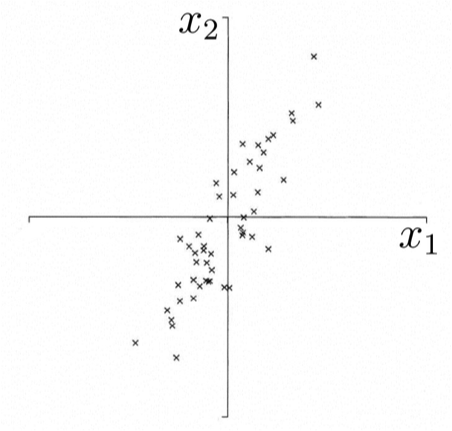
\includegraphics[scale=0.8]{img/pca.png}
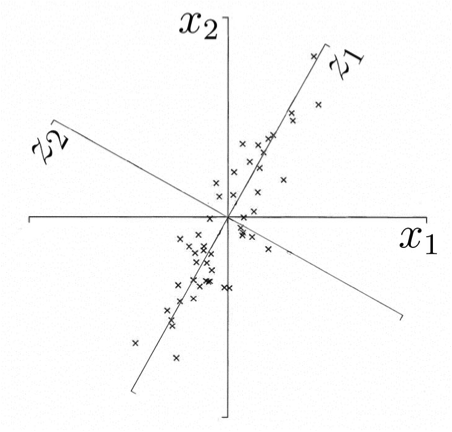
\includegraphics[scale=0.8]{img/pca1.png}
\label{pca}
\end{figure}
Immaginiamo di avere questi dati disposti in uno spazio bidimensionale (la PCA non si applica mai ad uno spazio bidimensionale in quanto non c'è nulla da ridurre). I dati sono disposti in modo tale che ci sia una varianza, inoltre questi dati potrebbero essere raggruppati in un cluster che potrebbe essere un ellisse. Supponiamo di sapere che questi dati appartengono a due cluster differenti. Allora qual'è il principio utilizzato per dividere questi dati? Esempio un metodo potrebbe essere quello di classificare tutti i pattern che rientrano nel primo quadrante e così via, quindi una classificazione che sta avvenendo sulla densità ovvero sulla distribuzione. Fondamentalmente questa suddivisione sta avvenendo in base alla varianza, questo si può spiegare perchè per i dati che si trovano intorno all'origine, soprattutto in prossimità della bisettrice tra il secondo e quarto quadrante, la varianza è molto piccola, mentre per gli altri, quelli che si trovano sulla bisettrice tra il primo ed il terzo quadrante la varianza più grande, quindi danno molta più informazione rispetto agli altri. Allora fatte queste osservazioni, quale potrebbe essere la trasformazione di un dataset in un altro dataset? Cioè l'operazione di proiettare tutti i vettori in un altro spazio, in questo caso nello spazio delle bisettrici, oppure equivalentemente nello spazio degli autovettori della matrice di covarianza dei dati. La matrice di covarianza ha sulla diagonale principale le varianze e al di fuori della diagonale principale ha le covarianze ovvero le correlazioni tra coppie di componenti. Sostanzialmente stiamo dicendo che se andiamo a vedere la matrice di covarianza (in questo caso è una matrice $2\times2$) osserviamo che sulla diagonale principale abbiamo la varianza sulla prima componente e sulla seconda componente, ci aspettiamo che una delle due sia maggiore dell'altra. 
Si tende a proiettare i pattern sulle due bisettrici, o equivalentemente gli autovettori della matrice di covarianza che corrispondono proprio ai due assi. Se riuscissi a proiettare, dopo aver calcolato gli autovettori della matrice di covarianza, alla fine identifico come componente  principale $z_1$, cioè quella a varianza maggiore, mentre come seconda componente principale prendo in considerazione $z_2$, cioè quella in cui la varianza tra le due è minore. Inoltre si conosce che le varianze della matrice di covarianza sono direttamente proporzionali agli autovalori della matrice di covarianza, quindi autovalori o varianze piò meno sono la stessa cosa. A questo punto il giochino facile è quello di prendere i dati, fare la matrice di covarianza, calcolare gli autovettori e gli autovalori, ordinare in ordine decrescente gli autovalori e corrispondentemente gli autovettori, scegliere gli autovalori maggiori e  ci si ferma quando la somma di questi autovalori supera una certa soglia. \'E ovvio che la somma degli autovalori non può essere maggiore di uno, di conseguenza se ipotizziamo di volere l'$80\%$ d'informazione allora sulla somma totale degli autovalori devo prendere tanti autovalori che sommati non superano 0.8. Così mi scelgo $k$ componenti principali tale che $\sum_{i=1}^k \lambda_i \leq 0.8$. Dove $k$ rappresenta il numero di componenti principali che seleziono in corrispondenza di questi autovalori, quindi ho $k$ autovettori che sono i nuovi assi del nuovo spazio sul quale vado a proiettare i pattern. I pattern erano in $d$ dimensioni e adesso sono proiettati su $k$ dimensioni per cui i pattern divetano $k$ dimensionali. Qual'è il vantaggio? se io ho pattern a cento dimensioni e scopro che la maggiore informazione è concentrata nelle prime dieci componenti principali allora ho ridotto lo spazio da cento dimensioni in pattern di dimensione dieci, conservando l'$80\%$ dell'informazione. Tutto ciò ha una base teorica:\\

\noindent Preso un pattern di $p$ variabili $\mathbf{x} = \{x_1, \dots, x_p\}$ vogliamo calcolare la prima componente principale dell'insieme dei campioni come trasformazione lineare di $\mathbf{x}$ tale che $z_1$ abbia la maggiore informazione (o che la varianza sia massima), quindi possiamo scrivere
\begin{equation}\label{70}
z_1 = \mathbf{a}_1^T \mathbf{x} = \sum_{i=1}^p \mathbf{a}_{i1} x_i
\end{equation}
dove il vettore $\mathbf{a}_1 = \{ a_{11}, a_{21}, \dots, a_{p1}\}$, è il vettore di pesi. 
Questo è un problema di ottimizzazione, perchè ancora una volta lo scopo principale è quello di massimizzare. Di conseguenza se voglio trovare la $k$-esima componente principale allora la \ref{70} diventa
\begin{equation}
z_k = \mathbf{a}_k^T \mathbf{x} \quad \quad \quad k=1, \dots, p
\end{equation}
dove il vettore $\mathbf{a}_k = \{ a_{1k}, a_{2k}, \dots, a_{pk} \}$, come prima è il vettore dei pesi.
Naturalmente le componenti principali calcolate devono essere relative alle componenti principali precedenti. Quindi non solo vogliamo che la varianza di $z_k$ sia massima, ma vogliamo anche che la covarianza di $z_k$ e $z_l$ con $1 \leq l < k$ sia uguale a zero, cioè fondamentalmente che non ci sia correlazione. Oltre alle componenti principali in senso di massimizzare la varianza, un altro vincolo è quello di avere componenti scorrelate fra di loro. Un ulteriore condizione è che $\mathbf{a}_k^T \mathbf{a}_k  =1 $. Adesso vediamo come trovare la prima componente principale. La varianza di $z_1$ la possiamo anche scrivere mediante una forma altrenativa, cioè
\begin{equation}\label{72}
var(z_1) = E[z_1^2] - E[z_2]^2
\end{equation}
dove $E$ sta ad indicare la media. Dalla \ref{70} sappiamo che $z_1 = \mathbf{a}_1^T \mathbf{x}$, quindi $x_1^2$ equivale a moltiplicare
\begin{equation}
\begin{split}
z_1^2 &= \mathbf{a}_1^T\mathbf{x} \cdot \mathbf{a}_1^T\mathbf{x}\\
&= \sum_{i=1}^p \mathbf{a}_{i1} x_i \sum_{j=1}^p \mathbf{a}_{j1} x_j\\
&= \sum_{i,j=1}^p \mathbf{a}_{i1} \mathbf{a}_{j1} \mathbf{x}_i \mathbf{x}_j\\
\end{split}
\end{equation}
dato che stiamo calcolando la media di $z_1^2$ possiamo scrivere che
\begin{equation}
E[z_1^2] = \sum_{i,j=1}^p \mathbf{a}_{i1} \mathbf{a}_{j1} E[\mathbf{x}_i \mathbf{x}_j]
\end{equation}
Facciamo la stessa cosa per $E[z_2]^2$, ma questa volta calcoliamo il quadrato della madia quindi facendo le opportune moltiplicazioni otteniamo
\begin{equation}
\sum_{i,j=1}^p \mathbf{a}_{i1} \mathbf{a}_{j1} E[\mathbf{x}_i] E[\mathbf{x}_j]
\end{equation}
andando a sostituire nella \ref{72} i valori ottenuti per $E[z_1^2]$ e $[z_1]^2$ otteniamo
\begin{equation}
var(z_1) = \sum_{i,j=1}^p \mathbf{a}_{i1} \mathbf{a}_{j1} E[\mathbf{x}_i \mathbf{x}_j] - \sum_{i,j=1}^p \mathbf{a}_{i1} \mathbf{a}_{j1} E[\mathbf{x}_i] E[\mathbf{x}_j]
\end{equation}
a questo punto metto in evidenza la doppia sommatoria
\begin{equation}\label{76}
\sum_{i,j=1}^p \mathbf{a}_{i1} \mathbf{a}_{j1} \mathbf{S}_{ij} 
\end{equation}
dove $\mathbf{S}_{ij} = \sigma_{x_i,x_j}= E[\mathbf{x}_i \mathbf{x}_j] - E[\mathbf{x}_i] E[\mathbf{x}_j]$, $\mathbf{S}$ è la matrice di covarianza, quindi $\mathbf{S}_{ij}$ è l'elemento della matrice di covarianza. 
La \ref{76} può essere scritta come 
\begin{equation}
var(z_1) = \mathbf{a}_1^T \mathbf{S}\mathbf{a}_1
\end{equation}
A questo punto il problema è quello di massimizzare la varianza di $z_1$, quindi bisogna massimizzare  $var(z_1) = \mathbf{a}_1^T \mathbf{S}\mathbf{a}_1$ soggetto a $\mathbf{a}_1^T \mathbf{a}_1  = 1$. In questo caso si utilizza la teoria della regolarizzazione, fondamentalmente si utilizza il moltiplicatore di lagrange che porta il vincolo nella funzione obiettivo. In questo caso, dato che ho il vincolo $\mathbf{a}_1^T \mathbf{a}_1  = 1$ allora voglio che $\mathbf{a}_1^T \mathbf{a}_1  -1= 0$, data questa condizione allora è ovvio che $\mathbf{a}_1^T \mathbf{a}_1$ deve essere uguale ad uno. A questo punto devo massimizzare la funzione obiettivo che è  $\mathbf{a}_1^T \mathbf{S}\mathbf{a}_1$ più il vincolo,  ma poichè sto massimizzando allora devo massimizzare $-\mathbf{a}_1^T \mathbf{a}_1$, quindi
\begin{equation}
\mathbf{a}_1^T \mathbf{S}\mathbf{a}_1 + ( - \mathbf{a}_1^T \mathbf{a}_1  - 1)
\end{equation}
alla fine mi viene 
\begin{equation}
\mathbf{a}_1^T \mathbf{S}\mathbf{a}_1 - \mathbf{a}_1^T \mathbf{a}_1  -1 
\end{equation}
ovviamente la prima  parte è la funzione obiettivo originale, mentre la seconda parte è il vincolo che sto aggiungendo, a cui devo dare un peso $\lambda$ che prende il nome di moltiplicatore di lagrange
\begin{equation}
 \mathbf{a}_1^T \mathbf{S}\mathbf{a}_1 - \lambda(\mathbf{a}_1^T \mathbf{a}_1  -1)
\end{equation}
con $0 < \lambda \leq 1$. A questo punto è facile, come si trova il massimo di una funzione? derivata prima uguale a zero. Qual'è il valore per cui voglio ottenere il massimo? \'E $\mathbf{a}_1$. Perchè $\lambda$ lo fisso, $\mathbf{S}$ è la matrice di covarianza dei dati, quindi faccio la derivata rispetto ad $\mathbf{a}_1$, quindi pongo tutto uguale a zero
\begin{equation}
\mathbf{S}\mathbf{a}_1 - \lambda \mathbf{a}_1 = 0
\end{equation}
metto in evidenza $\mathbf{a}_1$
\begin{equation}
(\mathbf{S}-\lambda \mathbf{I}_p)\mathbf{a_1} = 0
\end{equation}
in questa equazione $\lambda$ è l'autovalore della matrice di covarianza e $\mathbf{a}_1$ non è altro che l'autovettore corrispondente.\\

\noindent Fin qui abbiamo massimizzato la varianza sulla prima componente principale, quindi $\lambda$ corrisponde all'autovalore maggiore, cioè sto massimizzando la varianza della prima componente principale, quindi fondamentalmente sto trovando la componente principale per la quale ho la massima varianza, massima varianza equivale a dire massimo autovalore. Quindi riassumendo, presi i dati, mi calcolo la matrice di covarianza $\mathbf{S}$, mi calcolo gli autovalori e gli autovettori della matrice di covarianza, il primo autovalore corrisponde alla massima varianza e l'autovettore corrispondente alla prima componente principale.\\
A questo punto ho calcolato $\mathbf{a}_1$ ma dalla \ref{70} dobbiamo ricavarci $z_1$ quindi moltiplicando $\mathbf{a}_1^T \mathbf{x}$ non faccio altro che la proiezione di $\mathbf{x}$ su $\mathbf{a}_1$ (il prodotto interno $\mathbf{a}_1^T \mathbf{x}$ non è altro che la proiezione di $\mathbf{x}$ su $\mathbf{a}_1$). \\
Quindi possiamo dire che la varianza della prima componente principale corrisponde all'autovalore maggiore. Dimostriamolo:
Traduciamo formalmente quello che abbiamo detto, quindi la varianza della prima componete è uguale al primo autovalore che corrisponde a quello maggiore
\begin{equation}\label{104}
var(z_1) = \lambda_1
\end{equation}
quindi dall'equazione
\begin{equation}
(\mathbf{S}-\lambda \mathbf{I}_p)\mathbf{a_1} = 0
\end{equation}
effettuando alcuni semplici passaggi matematici
\begin{equation}
\begin{split}
\mathbf{S}\mathbf{a}_1 - \lambda \mathbf{a}_1 &= 0 \\
\mathbf{S}\mathbf{a}_1 &=  \lambda \mathbf{a}_1\\ 
\mathbf{a}_1^T  \cdot \mathbf{S}\mathbf{a}_1 &=  \lambda \mathbf{a}_1 \cdot \mathbf{a}_1^T\\
\mathbf{a}_1^T\mathbf{S}\mathbf{a}_1 &=  \lambda \mathbf{a}_1^T\mathbf{a}_1\\
\mathbf{a}_1^T\mathbf{S}\mathbf{a}_1 &=  \lambda
\end{split}
\end{equation}
dato che $\mathbf{a}_1^T\mathbf{a}_1 =  1$ e $var(z1) = \mathbf{a}_1^T\mathbf{S}\mathbf{a}_1$, quindi è dimostrata la \ref{104}.\\


\noindent Ho trovato la prima componente principale corrispondente all' autovettore corrispondete all'autovalore maggiore cioè alla varianza maggiore, che in modo geometrico corrisponde alla proiezione di $\mathbf{x}$ sull'asse maggiore dell'ellissoide che circoscrive i dati.\\

\noindent La seconda componente principale come la calcolo? Massimizzando la varianza $z_2$ ma questa volta con il vincolo $\mathbf{a}_2^T\mathbf{a}_2 = 1$ quindi ho di nuovo 
\begin{equation}
 \mathbf{a}_2^T \mathbf{S}\mathbf{a}_2 - \lambda(\mathbf{a}_2^T \mathbf{a}_2  -1)
\end{equation}
solo che però voglio anche che la covarianza della seconda componente principale rispetto alla prima componente principale sia uguale a zero (che siano scorrelate). Allora si introduce un altro paramentro 
\begin{equation}
cov(z_2,z_1) = \mathbf{a}_1^T\mathbf{S}\mathbf{a}_2 = \lambda_1\mathbf{a}_1^T\mathbf{a}_2
\end{equation}
La $cov(z_2, z_1) = \mathbf{a}_1^T\mathbf{S}\mathbf{a}_2$ quindi fondamentalmente sarebbe l'elemento $S_{21}$ della matrice di covarianza, quindi la posso scrivere o come $\mathbf{a}_1^T\mathbf{S}\mathbf{a}_2$ oppure equivalentemente che lo possiamo scrivere anche come $\lambda_1\mathbf{a}_1^T\mathbf{a}_2$
questo si può dimostrare come precedentemente, 
\begin{equation}
\mathbf{S}\mathbf{a}_2 = \lambda_1 \mathbf{a}_2
\end{equation}
moltiplico entrambi i membri per $\mathbf{a}_1^T$ ed ottengo
\begin{equation}
\mathbf{a}_1^T \cdot \mathbf{S}\mathbf{a}_2 = \lambda_1 \mathbf{a}_2 \cdot \mathbf{a}_1^T
\end{equation}
ottenendo così
\begin{equation}
\mathbf{a}_1^T \mathbf{S}\mathbf{a}_2 = \lambda_1  \mathbf{a}_1^T \mathbf{a}_2 
\end{equation}
ma $\mathbf{a}_1^T \mathbf{S}\mathbf{a}_2$ non è altro che la $cov(z_2, z_1)$ per cui abbiamo dimostrato che
\begin{equation}
cov(z_2, z_1) = \lambda_1  \mathbf{a}_1^T \mathbf{a}_2 
\end{equation}
A questo punto dobbiamo minimizzare la covarianza che come prima significa massimizzare meno la covarianza. Quindi è necessario massimizzare $- \lambda_1  \mathbf{a}_1^T \mathbf{a}_2$. Facciamo la derivata rispetto ad $\mathbf{a_2}$ la poniamo uguale a zero e calcoliamo $\mathbf{a_2}$. Questo procedimento viene effettuato per $\mathbf{a_3}, \mathbf{a_4}, \dots, \mathbf{a_n}$ ottenendo tutte le altre componenti principale. In generale si può definire 
\begin{equation}
var(z_k) = \mathbf{a_k}^T \mathbf{S} \mathbf{a_k}
\end{equation}
che è uguale al k-esimo autovalore nell'ordine discendente, quindi dall'autovalore più grande all'autovalore più piccolo della matrice di covarianza. La k-esima componente principale trattiene la frazione maggiore della variazione del dataset dei campioni. 


%
